\documentclass{article}

%% Page Margins %%
\usepackage{geometry}
\geometry{
    top = 0.75in,
    bottom = 0.75in,
    right = 0.75in,
    left = 0.75in,
}

\usepackage{amsmath}
\usepackage{graphicx}
\usepackage{parskip}

\title{Assembly Project: Breakout}

% TODO: Enter your name
\author{Aviraj Newatia}

\begin{document}
\maketitle

\section{Instruction and Summary}

\begin{enumerate}

    \item Which milestones were implemented? 
    % TODO: List the milestone(s) and in the case of 
    %       Milestones 4 & 5, list what features you 
    %       implemented, sorted into easy and hard 
    %       categories.
    \begin{itemize}
    \item   Milestone 1
    \item   Milestone 2
    \item   Milestone 3
    \item   Milestone 4:
    \begin{itemize}
        \item Launching the ball (spacebar) and moving the initial location of the paddle and ball ('a' and 'd')
        \item Pausing the game ('p') and Resuming (spacebar or 'p')
        \item Ball Speed Increases on Hit
        \item Restart game at any point, even after losing ('r')
    \end{itemize}
    \item Milestone 5:
    \begin{itemize}
        \item Animated Brick Breaking and Colour Changing
        \item Multiple-Hit Bricks
        \item Sound Effects
    \end{itemize}
    \end{itemize}

    \item How to view the game:
    % TODO: specify the pixes/unit, width and height of 
    %       your game, etc.  NOTE: list these details in
    %       the header of your breakout.asm file too!
    
    \begin{enumerate}

    \item Height 128
    \item Width 64
    \item Height Unit 2
    \item Width Unit 2


    \end{enumerate}

    

\begin{figure}[ht!]
    \centering
    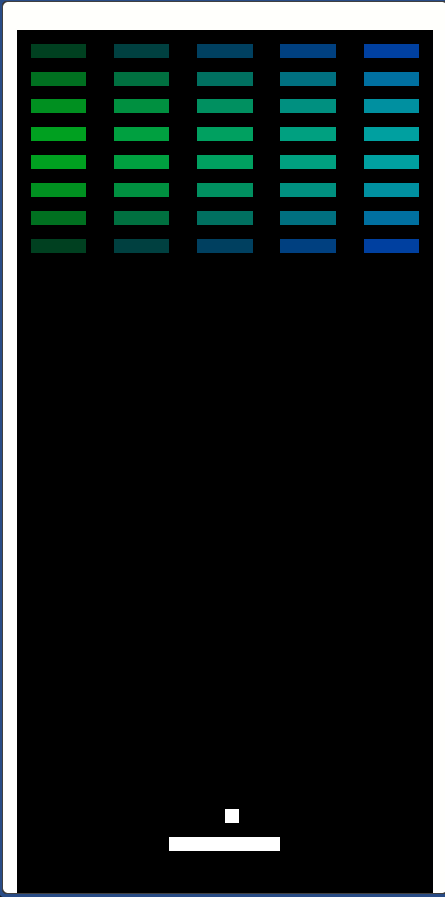
\includegraphics[width=0.3\textwidth]{scene.png}
    \caption{The initial screen for Breakout.}
    \label{Instructions}
\end{figure}

\item Game Summary:
% TODO: Tell us a little about your game.
\begin{itemize}
\item My game is a rendition of breakout, the classic arcade game. The goal of the game is to break all of the blocks on the screen using the ball which is controlled by bouncing it off of a movable paddle. In this game there is a single level with 40 bricks to break, some of which require multiple hits to destroy. After the first hit on these multi-hit bricks, they turn grey. After the second hit they are destroyed. Whenever a brick is hit, a sound is played to signify the collision, and the colour change or destruction of the brick is animated. At the beginning of the game, you can move the initial location of the paddle and the ball and then press space to launch/start the game. At any point, you can press 'p' to pause the game and then spacebar to resume it. You can also press 'r' at any point to restart the game or press 'q' to quit. If the ball falls below the paddle, the game ends, at which point you can press 'r' to restart or 'q' to quit. If you break all of the bricks, you win the game and can press 'r' to restart or 'q' to quit.
\end{itemize}

    
\end{enumerate}

\section{Attribution Table}
% TODO: If you worked in partners, tell us who was 
%       responsible for which features. Some reweighting 
%       might be possible in cases where one group member
%       deserves extra credit for the work they put in.

\begin{center}
\begin{tabular}{|| c ||}
\hline
 Student 1 (Aviraj Newatia 1007837708) \\ 
 \hline
 Everything, my nonexistent partner didn't help at all \\ 
 \hline
\end{tabular}
\end{center}

My game functions with 4 main game loops, 'game\_loop' which is enacted when the game first starts allowing the player to move the initial location of the paddle and ball and launch the ball to start the game. 'paused\_game\_loop' is reached when the player pauses the game, and allows the player to resume or exit the game from that state. 
The third game loop is the 'moving\_game\_loop' which is the main actual "playing" game loop in which the ball is moved and all regular playing controls are bound to the handle\_keyboard function. The last game loops is the 'exit\_loop' which is a game loop which is reached when the ball falls below the paddle. This game loop exists to allow the player to restart or quit the game.
Each of these game loops needs its own keyboard handling function so that only certain controls work in each situation. I could have designed a single keyboard handling function and checked where I came from, but this allowed me to minimize memory usage by increasing the manual logic performed using temporary registers and more lines of code. \\
The game plays a sound through syscalls, and the bricks are broken using loops that move left and right to remove coloured pixels and set them to black. The deletion functions also contain logic to check if the brick should be destroyed, or if its 'durability' should be reduced by colouring it grey first. \\
The game functions handle collisions through a filter system, which essentially does a binary search on the current memory and register values to determine how the ball collision should be handled. This allowed me to reuse a lot of my code in place of some more logic, and made the collision handling quite pretty and concise, as well as efficient. \\
The animation of the brick breaking or recolouring is done by using a sleep syscall whenever a brick colouring is done, which makes the destruction happen one pixel at a time, creating a ripple animation from the point of impact. \\
There's a reset variables function which is called when the game is restarted, which resets all of the memory locations and the required registers to their values before jumping the control flow back to the beginning of main, so that main functions properly to redraw the screen after first drawing the whole screen black again. \\


\end{document}